%%%%%
%%Title: HiPi+Bus V0.2 Chapter 7
%%Creator: Ando Ki
%%CreationDate: April 1992
%%FileName: sec4
%%RelatedFile: ch7
%%%%%
\section{TTL 신호의 전기적 규격}
TTL 신호의 전기적 규격은 {\tt <}표~\ref{table:ttl-spec}{\tt >}와 같다.
%
%
\begin{table}[htbp]
\caption{TTL 신호의 전기적 규격}\label{table:ttl-spec}
   \begin{center}
   \begin{tabular}{|l l|l|} \hline
	$V_t$    & typical & 2.5V\\
	$V_{OH}$ & min     & 2.0V\\
	$V_{IH}$ & max     & 1.8V\\
	$V_{IL}$ & min     & 0.8V\\
	$V_{OL}$ & max     & 0.6V\\
	$GND$    &         & 0.0V\\ \hline
   \end{tabular}
   \end{center}
\end{table}
%

%
신호의 참조전압을 GND 0V라 하고, 터미네이션에 의한 전압이 $V_t$이고,
신호가 구동되지 않은 상태에서의 신호선의 전압은 $V_{OH}^{min}$ 이상이 되어야 하고,
신호선에 신호를 구동할 때 구동소자는 해당 신호선의 전압을 $V_{OL}^{max}$와
$V_{OL}^{min}$ 사이가 되도록 해야 한다.
수신소자의 경우는 $V_{IH}^{min}$ 이상이 되는 전압에 대해서는 높은 전압으로,
$V_{IL}^{max}$ 이하의 전압에 대해서는 낮은 전압으로 받아들여야 한다.
이것을 그림으로 나타내면 {\tt <}그림~\ref{figure:signal-spec-ttl}{\tt >}과 같다.
%
\begin{figure}[htb]
    \centerline{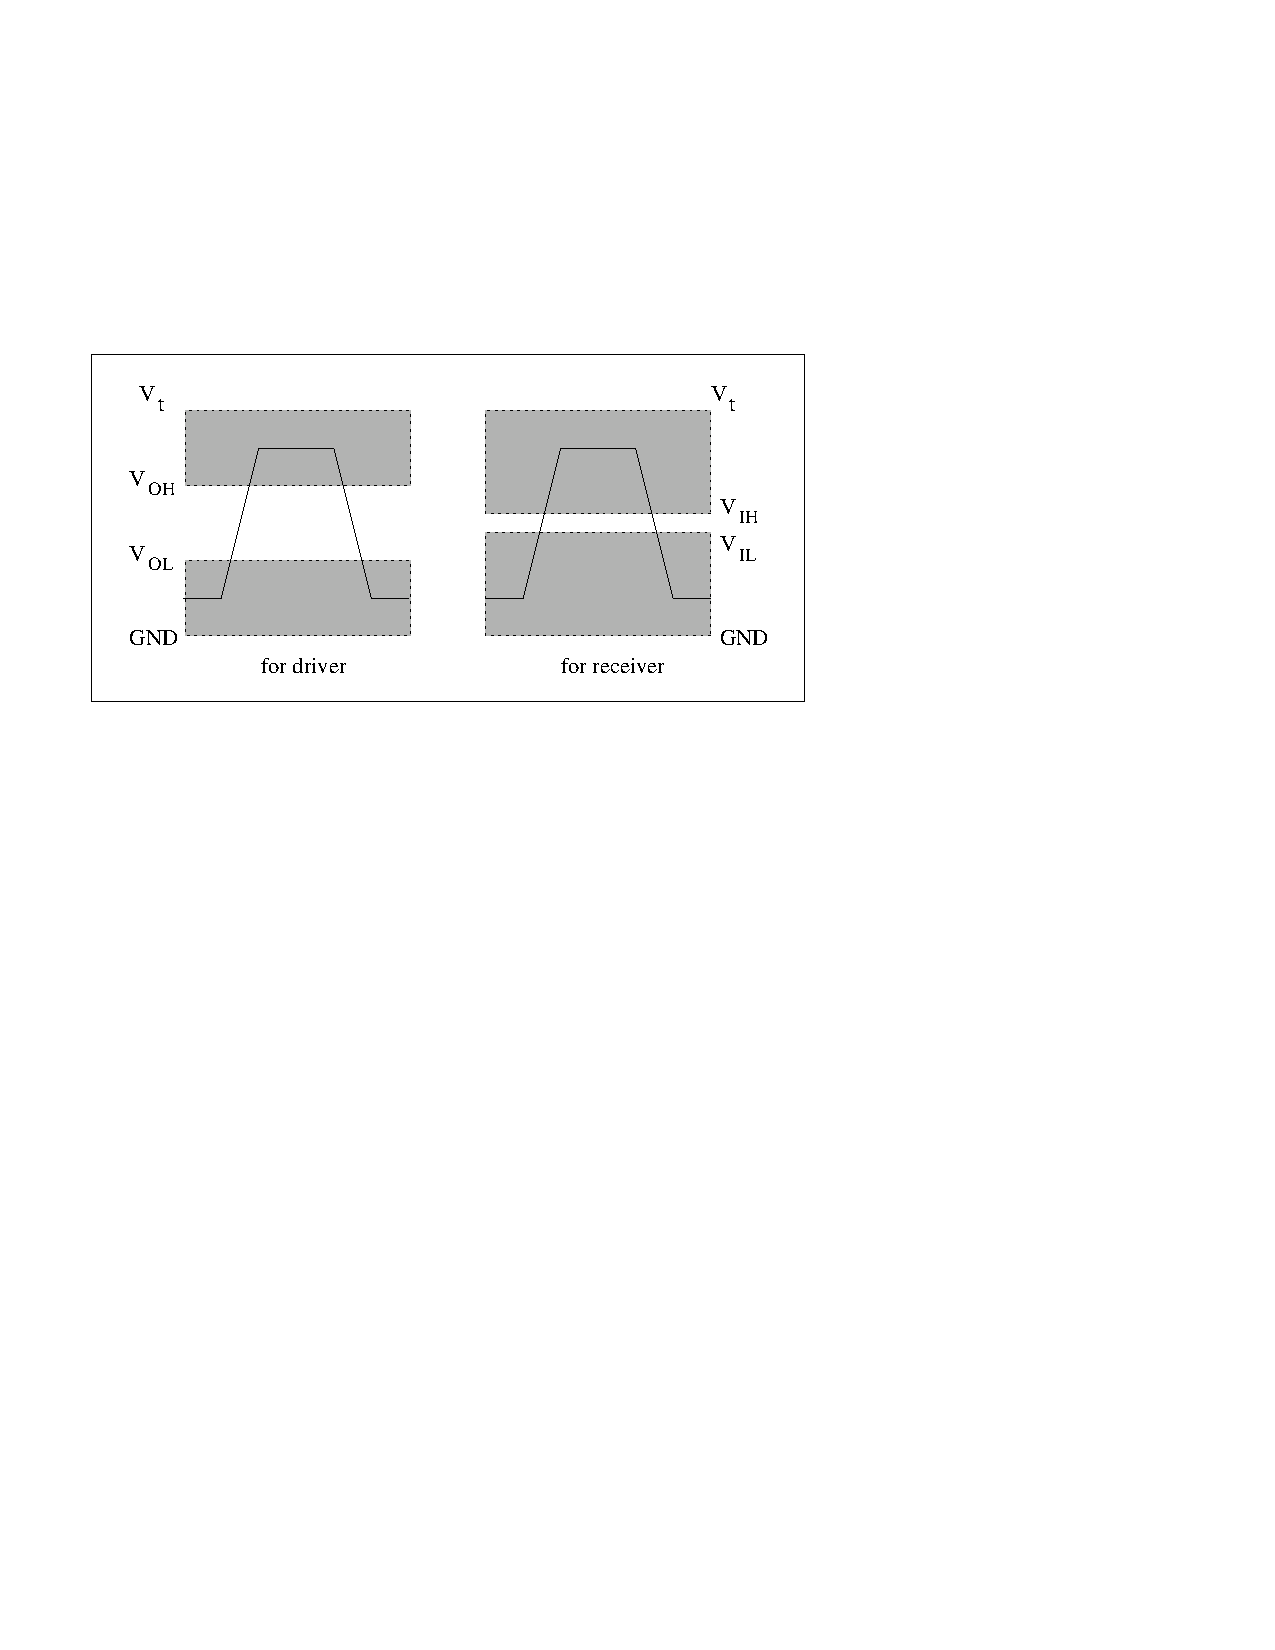
\includegraphics{ch7/FIG/signal-spec.jpg}}
   \caption{TTL 신호선의 전기적 규격}\label{figure:signal-spec-ttl}
\end{figure}
%

\subsection{인터페이스 회로의 용량성 부하}
%
TTL 버스에 연결되는 수신소자(receiver), 구동소자(driver), 수신/구동소자(transceiver)의
각 출력단의 용량성 부하는 15$p$F보다 크지 않아야 한다.

\subsection{구동소자의 종류}
TTL 구동소자의 종류는 totem-pol, three-state, 그리고 open-collector 등
세가지가 있다.
%
%%%%%
%\end{document}
%%%%%
